\documentclass[twoside]{book}

% Packages required by doxygen
\usepackage{fixltx2e}
\usepackage{calc}
\usepackage{doxygen}
\usepackage[export]{adjustbox} % also loads graphicx
\usepackage{graphicx}
\usepackage[utf8]{inputenc}
\usepackage{makeidx}
\usepackage{multicol}
\usepackage{multirow}
\PassOptionsToPackage{warn}{textcomp}
\usepackage{textcomp}
\usepackage[nointegrals]{wasysym}
\usepackage[table]{xcolor}

% Font selection
\usepackage[T1]{fontenc}
\usepackage[scaled=.90]{helvet}
\usepackage{courier}
\usepackage{amssymb}
\usepackage{sectsty}
\renewcommand{\familydefault}{\sfdefault}
\allsectionsfont{%
  \fontseries{bc}\selectfont%
  \color{darkgray}%
}
\renewcommand{\DoxyLabelFont}{%
  \fontseries{bc}\selectfont%
  \color{darkgray}%
}
\newcommand{\+}{\discretionary{\mbox{\scriptsize$\hookleftarrow$}}{}{}}

% Page & text layout
\usepackage{geometry}
\geometry{%
  a4paper,%
  top=2.5cm,%
  bottom=2.5cm,%
  left=2.5cm,%
  right=2.5cm%
}
\tolerance=750
\hfuzz=15pt
\hbadness=750
\setlength{\emergencystretch}{15pt}
\setlength{\parindent}{0cm}
\setlength{\parskip}{0.2cm}
\makeatletter
\renewcommand{\paragraph}{%
  \@startsection{paragraph}{4}{0ex}{-1.0ex}{1.0ex}{%
    \normalfont\normalsize\bfseries\SS@parafont%
  }%
}
\renewcommand{\subparagraph}{%
  \@startsection{subparagraph}{5}{0ex}{-1.0ex}{1.0ex}{%
    \normalfont\normalsize\bfseries\SS@subparafont%
  }%
}
\makeatother

% Headers & footers
\usepackage{fancyhdr}
\pagestyle{fancyplain}
\fancyhead[LE]{\fancyplain{}{\bfseries\thepage}}
\fancyhead[CE]{\fancyplain{}{}}
\fancyhead[RE]{\fancyplain{}{\bfseries\leftmark}}
\fancyhead[LO]{\fancyplain{}{\bfseries\rightmark}}
\fancyhead[CO]{\fancyplain{}{}}
\fancyhead[RO]{\fancyplain{}{\bfseries\thepage}}
\fancyfoot[LE]{\fancyplain{}{}}
\fancyfoot[CE]{\fancyplain{}{}}
\fancyfoot[RE]{\fancyplain{}{\bfseries\scriptsize Generated on Tue Mar 29 2016 00\+:57\+:50 for Laser pointer (client) by Doxygen }}
\fancyfoot[LO]{\fancyplain{}{\bfseries\scriptsize Generated on Tue Mar 29 2016 00\+:57\+:50 for Laser pointer (client) by Doxygen }}
\fancyfoot[CO]{\fancyplain{}{}}
\fancyfoot[RO]{\fancyplain{}{}}
\renewcommand{\footrulewidth}{0.4pt}
\renewcommand{\chaptermark}[1]{%
  \markboth{#1}{}%
}
\renewcommand{\sectionmark}[1]{%
  \markright{\thesection\ #1}%
}

% Indices & bibliography
\usepackage{natbib}
\usepackage[titles]{tocloft}
\setcounter{tocdepth}{3}
\setcounter{secnumdepth}{5}
\makeindex

% Hyperlinks (required, but should be loaded last)
\usepackage{ifpdf}
\ifpdf
  \usepackage[pdftex,pagebackref=true]{hyperref}
\else
  \usepackage[ps2pdf,pagebackref=true]{hyperref}
\fi
\hypersetup{%
  colorlinks=true,%
  linkcolor=blue,%
  citecolor=blue,%
  unicode%
}

% Custom commands
\newcommand{\clearemptydoublepage}{%
  \newpage{\pagestyle{empty}\cleardoublepage}%
}


%===== C O N T E N T S =====

\begin{document}

% Titlepage & ToC
\hypersetup{pageanchor=false,
             bookmarks=true,
             bookmarksnumbered=true,
             pdfencoding=unicode
            }
\pagenumbering{roman}
\begin{titlepage}
\vspace*{7cm}
\begin{center}%
{\Large Laser pointer (client) \\[1ex]\large 0.\+3 }\\
\vspace*{1cm}
{\large Generated by Doxygen 1.8.10}\\
\vspace*{0.5cm}
{\small Tue Mar 29 2016 00:57:50}\\
\end{center}
\end{titlepage}
\clearemptydoublepage
\tableofcontents
\clearemptydoublepage
\pagenumbering{arabic}
\hypersetup{pageanchor=true}

%--- Begin generated contents ---
\chapter{R\+E\+A\+D\+M\+E}
\label{md_doc__r_e_a_d_m_e}
\hypertarget{md_doc__r_e_a_d_m_e}{}
No graph are present in this doc, but you can get them by generating the doc with our doxyfile included with the source code. 
\chapter{Namespace Index}
\section{Namespace List}
Here is a list of all namespaces with brief descriptions\+:\begin{DoxyCompactList}
\item\contentsline{section}{\hyperlink{namespace_ui}{Ui} }{\pageref{namespace_ui}}{}
\end{DoxyCompactList}

\chapter{Hierarchical Index}
\section{Class Hierarchy}
This inheritance list is sorted roughly, but not completely, alphabetically\+:\begin{DoxyCompactList}
\item \contentsline{section}{message}{\pageref{structmessage}}{}
\item Q\+Dialog\begin{DoxyCompactList}
\item \contentsline{section}{Settings\+Dialog}{\pageref{class_settings_dialog}}{}
\end{DoxyCompactList}
\item Q\+Graphics\+Scene\begin{DoxyCompactList}
\item \contentsline{section}{custom\+\_\+scene}{\pageref{classcustom__scene}}{}
\end{DoxyCompactList}
\item Q\+Main\+Window\begin{DoxyCompactList}
\item \contentsline{section}{Main\+Window}{\pageref{class_main_window}}{}
\end{DoxyCompactList}
\item \contentsline{section}{Settings\+Dialog\+:\+:Settings}{\pageref{struct_settings_dialog_1_1_settings}}{}
\end{DoxyCompactList}

\chapter{Class Index}
\section{Class List}
Here are the classes, structs, unions and interfaces with brief descriptions\+:\begin{DoxyCompactList}
\item\contentsline{section}{\hyperlink{classcustom__scene}{custom\+\_\+scene} }{\pageref{classcustom__scene}}{}
\item\contentsline{section}{\hyperlink{class_main_window}{Main\+Window} }{\pageref{class_main_window}}{}
\item\contentsline{section}{\hyperlink{structmessage}{message} }{\pageref{structmessage}}{}
\item\contentsline{section}{\hyperlink{struct_settings_dialog_1_1_settings}{Settings\+Dialog\+::\+Settings} }{\pageref{struct_settings_dialog_1_1_settings}}{}
\item\contentsline{section}{\hyperlink{class_settings_dialog}{Settings\+Dialog} }{\pageref{class_settings_dialog}}{}
\end{DoxyCompactList}

\chapter{File Index}
\section{File List}
Here is a list of all files with brief descriptions\+:\begin{DoxyCompactList}
\item\contentsline{section}{\hyperlink{custom__scene_8cpp}{custom\+\_\+scene.\+cpp} }{\pageref{custom__scene_8cpp}}{}
\item\contentsline{section}{\hyperlink{custom__scene_8h}{custom\+\_\+scene.\+h} }{\pageref{custom__scene_8h}}{}
\item\contentsline{section}{\hyperlink{main_8cpp}{main.\+cpp} }{\pageref{main_8cpp}}{}
\item\contentsline{section}{\hyperlink{mainwindow_8cpp}{mainwindow.\+cpp} }{\pageref{mainwindow_8cpp}}{}
\item\contentsline{section}{\hyperlink{mainwindow_8h}{mainwindow.\+h} }{\pageref{mainwindow_8h}}{}
\item\contentsline{section}{\hyperlink{protocol_8cpp}{protocol.\+cpp} }{\pageref{protocol_8cpp}}{}
\item\contentsline{section}{\hyperlink{protocol_8h}{protocol.\+h} }{\pageref{protocol_8h}}{}
\item\contentsline{section}{\hyperlink{settingsdialog_8cpp}{settingsdialog.\+cpp} }{\pageref{settingsdialog_8cpp}}{}
\item\contentsline{section}{\hyperlink{settingsdialog_8h}{settingsdialog.\+h} }{\pageref{settingsdialog_8h}}{}
\end{DoxyCompactList}

\chapter{Namespace Documentation}
\hypertarget{namespace_ui}{}\section{Ui Namespace Reference}
\label{namespace_ui}\index{Ui@{Ui}}

\chapter{Class Documentation}
\hypertarget{classcustom__scene}{}\section{custom\+\_\+scene Class Reference}
\label{classcustom__scene}\index{custom\+\_\+scene@{custom\+\_\+scene}}


{\ttfamily \#include $<$custom\+\_\+scene.\+h$>$}



Inheritance diagram for custom\+\_\+scene\+:
\nopagebreak
\begin{figure}[H]
\begin{center}
\leavevmode
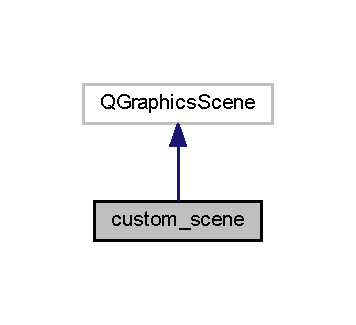
\includegraphics[width=171pt]{classcustom__scene__inherit__graph}
\end{center}
\end{figure}


Collaboration diagram for custom\+\_\+scene\+:
\nopagebreak
\begin{figure}[H]
\begin{center}
\leavevmode
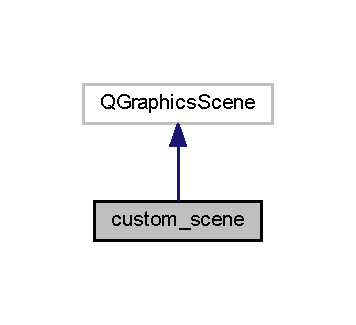
\includegraphics[width=171pt]{classcustom__scene__coll__graph}
\end{center}
\end{figure}
\subsection*{Public Slots}
\begin{DoxyCompactItemize}
\item 
void \hyperlink{classcustom__scene_aeb8481fa02536d26b015722df86f7800}{got\+New\+Position} (int x, int y)
\end{DoxyCompactItemize}


\subsection{Detailed Description}
\begin{DoxyAuthor}{Author}
Quentin Berdal Class Q\+Graphics\+Scene with mouse tracking. 
\end{DoxyAuthor}


Definition at line 13 of file custom\+\_\+scene.\+h.



\subsection{Member Function Documentation}
\hypertarget{classcustom__scene_aeb8481fa02536d26b015722df86f7800}{}\index{custom\+\_\+scene@{custom\+\_\+scene}!got\+New\+Position@{got\+New\+Position}}
\index{got\+New\+Position@{got\+New\+Position}!custom\+\_\+scene@{custom\+\_\+scene}}
\subsubsection[{got\+New\+Position}]{\setlength{\rightskip}{0pt plus 5cm}void custom\+\_\+scene\+::got\+New\+Position (
\begin{DoxyParamCaption}
\item[{int}]{x, }
\item[{int}]{y}
\end{DoxyParamCaption}
)\hspace{0.3cm}{\ttfamily [slot]}}\label{classcustom__scene_aeb8481fa02536d26b015722df86f7800}


Definition at line 3 of file custom\+\_\+scene.\+cpp.



The documentation for this class was generated from the following files\+:\begin{DoxyCompactItemize}
\item 
\hyperlink{custom__scene_8h}{custom\+\_\+scene.\+h}\item 
\hyperlink{custom__scene_8cpp}{custom\+\_\+scene.\+cpp}\end{DoxyCompactItemize}

\hypertarget{class_main_window}{}\section{Main\+Window Class Reference}
\label{class_main_window}\index{Main\+Window@{Main\+Window}}


{\ttfamily \#include $<$mainwindow.\+h$>$}



Inheritance diagram for Main\+Window\+:
\nopagebreak
\begin{figure}[H]
\begin{center}
\leavevmode
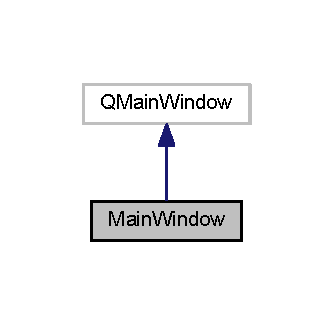
\includegraphics[width=160pt]{class_main_window__inherit__graph}
\end{center}
\end{figure}


Collaboration diagram for Main\+Window\+:
\nopagebreak
\begin{figure}[H]
\begin{center}
\leavevmode
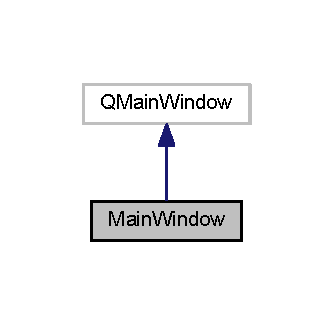
\includegraphics[width=160pt]{class_main_window__coll__graph}
\end{center}
\end{figure}
\subsection*{Public Slots}
\begin{DoxyCompactItemize}
\item 
void \hyperlink{class_main_window_a42f3e1ec38bdf049152b5bf0cf1e0fc6}{put\+Data} (\hyperlink{protocol_8h_ae5051f6f612e6d4218717f733bc50667}{Message} $\ast$data)
\begin{DoxyCompactList}\small\item\em Put data on serial port with protocol. $<$ See \char`\"{}protocol.\+h\char`\"{} for more information. \end{DoxyCompactList}\end{DoxyCompactItemize}
\subsection*{Signals}
\begin{DoxyCompactItemize}
\item 
\hyperlink{class_main_window_a4ed985f131d790a11639b39a0c5c75be}{position\+Updated} (int x, int y)
\end{DoxyCompactItemize}
\subsection*{Public Member Functions}
\begin{DoxyCompactItemize}
\item 
\hyperlink{class_main_window_a8b244be8b7b7db1b08de2a2acb9409db}{Main\+Window} (Q\+Widget $\ast$parent=0)
\item 
\hyperlink{class_main_window_ae98d00a93bc118200eeef9f9bba1dba7}{$\sim$\+Main\+Window} ()
\end{DoxyCompactItemize}


\subsection{Detailed Description}
Main G\+U\+I Contain all elements used to control the board 

Definition at line 30 of file mainwindow.\+h.



\subsection{Constructor \& Destructor Documentation}
\hypertarget{class_main_window_a8b244be8b7b7db1b08de2a2acb9409db}{}\index{Main\+Window@{Main\+Window}!Main\+Window@{Main\+Window}}
\index{Main\+Window@{Main\+Window}!Main\+Window@{Main\+Window}}
\subsubsection[{Main\+Window(\+Q\+Widget $\ast$parent=0)}]{\setlength{\rightskip}{0pt plus 5cm}Main\+Window\+::\+Main\+Window (
\begin{DoxyParamCaption}
\item[{Q\+Widget $\ast$}]{parent = {\ttfamily 0}}
\end{DoxyParamCaption}
)\hspace{0.3cm}{\ttfamily [explicit]}}\label{class_main_window_a8b244be8b7b7db1b08de2a2acb9409db}


Definition at line 9 of file mainwindow.\+cpp.

\hypertarget{class_main_window_ae98d00a93bc118200eeef9f9bba1dba7}{}\index{Main\+Window@{Main\+Window}!````~Main\+Window@{$\sim$\+Main\+Window}}
\index{````~Main\+Window@{$\sim$\+Main\+Window}!Main\+Window@{Main\+Window}}
\subsubsection[{$\sim$\+Main\+Window()}]{\setlength{\rightskip}{0pt plus 5cm}Main\+Window\+::$\sim$\+Main\+Window (
\begin{DoxyParamCaption}
{}
\end{DoxyParamCaption}
)}\label{class_main_window_ae98d00a93bc118200eeef9f9bba1dba7}


Definition at line 49 of file mainwindow.\+cpp.



\subsection{Member Function Documentation}
\hypertarget{class_main_window_a4ed985f131d790a11639b39a0c5c75be}{}\index{Main\+Window@{Main\+Window}!position\+Updated@{position\+Updated}}
\index{position\+Updated@{position\+Updated}!Main\+Window@{Main\+Window}}
\subsubsection[{position\+Updated}]{\setlength{\rightskip}{0pt plus 5cm}Main\+Window\+::position\+Updated (
\begin{DoxyParamCaption}
\item[{int}]{x, }
\item[{int}]{y}
\end{DoxyParamCaption}
)\hspace{0.3cm}{\ttfamily [signal]}}\label{class_main_window_a4ed985f131d790a11639b39a0c5c75be}


Here is the caller graph for this function\+:
\nopagebreak
\begin{figure}[H]
\begin{center}
\leavevmode
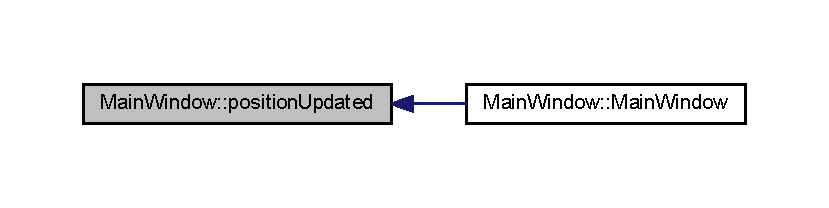
\includegraphics[width=350pt]{class_main_window_a4ed985f131d790a11639b39a0c5c75be_icgraph}
\end{center}
\end{figure}


\hypertarget{class_main_window_a42f3e1ec38bdf049152b5bf0cf1e0fc6}{}\index{Main\+Window@{Main\+Window}!put\+Data@{put\+Data}}
\index{put\+Data@{put\+Data}!Main\+Window@{Main\+Window}}
\subsubsection[{put\+Data}]{\setlength{\rightskip}{0pt plus 5cm}void Main\+Window\+::put\+Data (
\begin{DoxyParamCaption}
\item[{{\bf Message} $\ast$}]{data}
\end{DoxyParamCaption}
)\hspace{0.3cm}{\ttfamily [slot]}}\label{class_main_window_a42f3e1ec38bdf049152b5bf0cf1e0fc6}


Put data on serial port with protocol. $<$ See \char`\"{}protocol.\+h\char`\"{} for more information. 



Definition at line 159 of file mainwindow.\+cpp.



Here is the call graph for this function\+:
\nopagebreak
\begin{figure}[H]
\begin{center}
\leavevmode
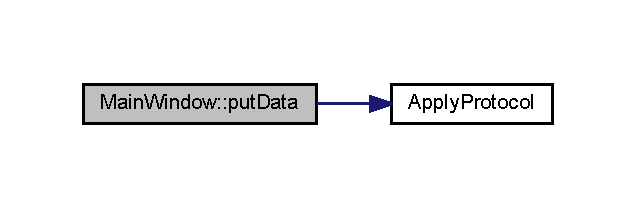
\includegraphics[width=305pt]{class_main_window_a42f3e1ec38bdf049152b5bf0cf1e0fc6_cgraph}
\end{center}
\end{figure}




The documentation for this class was generated from the following files\+:\begin{DoxyCompactItemize}
\item 
\hyperlink{mainwindow_8h}{mainwindow.\+h}\item 
\hyperlink{mainwindow_8cpp}{mainwindow.\+cpp}\end{DoxyCompactItemize}

\hypertarget{structmessage}{}\section{message Struct Reference}
\label{structmessage}\index{message@{message}}


{\ttfamily \#include $<$protocol.\+h$>$}

\subsection*{Public Attributes}
\begin{DoxyCompactItemize}
\item 
\hyperlink{protocol_8h_ad327bde01da3f3f8f71ae03db02572bc}{Protocol} \hyperlink{structmessage_a09bed901f53052cc020ab6ec8d64e3ee}{mode}
\item 
unsigned char $\ast$ \hyperlink{structmessage_a56cfb15f3cbc41b9b8e5e0ba34d6bea4}{data}
\begin{DoxyCompactList}\small\item\em Pointer to an array of data. \end{DoxyCompactList}\item 
unsigned int \hyperlink{structmessage_a3a17f9f2aa68b473300ae38d4bad06e8}{data\+\_\+size} =0
\begin{DoxyCompactList}\small\item\em Number of data in the array. \end{DoxyCompactList}\end{DoxyCompactItemize}


\subsection{Detailed Description}
Structure used by functions to read and write according to the protocol. You can interact with functions only through this structure. No verification is done on the struct, so be carefull when you assign data. Otherwise, you\textquotesingle{}ll send corrupted packet and the board will answer N\+A\+C\+K. 

Definition at line 38 of file protocol.\+h.



\subsection{Member Data Documentation}
\hypertarget{structmessage_a56cfb15f3cbc41b9b8e5e0ba34d6bea4}{}\index{message@{message}!data@{data}}
\index{data@{data}!message@{message}}
\subsubsection[{data}]{\setlength{\rightskip}{0pt plus 5cm}unsigned char$\ast$ message\+::data}\label{structmessage_a56cfb15f3cbc41b9b8e5e0ba34d6bea4}


Pointer to an array of data. 



Definition at line 42 of file protocol.\+h.

\hypertarget{structmessage_a3a17f9f2aa68b473300ae38d4bad06e8}{}\index{message@{message}!data\+\_\+size@{data\+\_\+size}}
\index{data\+\_\+size@{data\+\_\+size}!message@{message}}
\subsubsection[{data\+\_\+size}]{\setlength{\rightskip}{0pt plus 5cm}unsigned int message\+::data\+\_\+size =0}\label{structmessage_a3a17f9f2aa68b473300ae38d4bad06e8}


Number of data in the array. 



Definition at line 43 of file protocol.\+h.

\hypertarget{structmessage_a09bed901f53052cc020ab6ec8d64e3ee}{}\index{message@{message}!mode@{mode}}
\index{mode@{mode}!message@{message}}
\subsubsection[{mode}]{\setlength{\rightskip}{0pt plus 5cm}{\bf Protocol} message\+::mode}\label{structmessage_a09bed901f53052cc020ab6ec8d64e3ee}
Describe the type of packet. Accept A\+C\+K, N\+A\+C\+K, M\+O\+D\+E\+\_\+\+A\+U\+T\+O and M\+O\+D\+E\+\_\+\+T\+R\+A\+C\+K\+I\+N\+G 

Definition at line 40 of file protocol.\+h.



The documentation for this struct was generated from the following file\+:\begin{DoxyCompactItemize}
\item 
\hyperlink{protocol_8h}{protocol.\+h}\end{DoxyCompactItemize}

\hypertarget{struct_settings_dialog_1_1_settings}{}\section{Settings\+Dialog\+:\+:Settings Struct Reference}
\label{struct_settings_dialog_1_1_settings}\index{Settings\+Dialog\+::\+Settings@{Settings\+Dialog\+::\+Settings}}


{\ttfamily \#include $<$settingsdialog.\+h$>$}

\subsection*{Public Attributes}
\begin{DoxyCompactItemize}
\item 
Q\+String \hyperlink{struct_settings_dialog_1_1_settings_a973c8cfb942a512f34fc4227c0caa6dd}{name}
\begin{DoxyCompactList}\small\item\em Port name. \end{DoxyCompactList}\item 
qint32 \hyperlink{struct_settings_dialog_1_1_settings_ac19cc9431552857a75c657a464ba0700}{baud\+Rate}
\begin{DoxyCompactList}\small\item\em Baud rate. \end{DoxyCompactList}\item 
Q\+String \hyperlink{struct_settings_dialog_1_1_settings_a54e9d461f783386f314bc24b96665e53}{string\+Baud\+Rate}
\begin{DoxyCompactList}\small\item\em Baud rate to string. \end{DoxyCompactList}\item 
Q\+Serial\+Port\+::\+Data\+Bits \hyperlink{struct_settings_dialog_1_1_settings_a7dcd85d028a09508cb4567cf631b40e9}{data\+Bits}
\item 
Q\+String \hyperlink{struct_settings_dialog_1_1_settings_ab589b733b78af17744ab75067bfce051}{string\+Data\+Bits}
\item 
Q\+Serial\+Port\+::\+Parity \hyperlink{struct_settings_dialog_1_1_settings_ae08a00aa2e45218dade9046e3624cce7}{parity}
\item 
Q\+String \hyperlink{struct_settings_dialog_1_1_settings_aa2c662b2fb315f038e827d63d83b059b}{string\+Parity}
\item 
Q\+Serial\+Port\+::\+Stop\+Bits \hyperlink{struct_settings_dialog_1_1_settings_ab88ff384f7c1127bcbe2dd97b49696a4}{stop\+Bits}
\item 
Q\+String \hyperlink{struct_settings_dialog_1_1_settings_abde3c8410f779688ce6c2fcbbbb84f10}{string\+Stop\+Bits}
\item 
Q\+Serial\+Port\+::\+Flow\+Control \hyperlink{struct_settings_dialog_1_1_settings_aa962a6e7dbb8338af154305e4ff46cfc}{flow\+Control}
\item 
Q\+String \hyperlink{struct_settings_dialog_1_1_settings_a1b0a388ec5059bd2628acf9b7728f2f3}{string\+Flow\+Control}
\item 
bool \hyperlink{struct_settings_dialog_1_1_settings_ae1bfec3d6530f9791451d12aacfcb014}{local\+Echo\+Enabled}
\end{DoxyCompactItemize}


\subsection{Detailed Description}


Definition at line 26 of file settingsdialog.\+h.



\subsection{Member Data Documentation}
\hypertarget{struct_settings_dialog_1_1_settings_ac19cc9431552857a75c657a464ba0700}{}\index{Settings\+Dialog\+::\+Settings@{Settings\+Dialog\+::\+Settings}!baud\+Rate@{baud\+Rate}}
\index{baud\+Rate@{baud\+Rate}!Settings\+Dialog\+::\+Settings@{Settings\+Dialog\+::\+Settings}}
\subsubsection[{baud\+Rate}]{\setlength{\rightskip}{0pt plus 5cm}qint32 Settings\+Dialog\+::\+Settings\+::baud\+Rate}\label{struct_settings_dialog_1_1_settings_ac19cc9431552857a75c657a464ba0700}


Baud rate. 



Definition at line 28 of file settingsdialog.\+h.

\hypertarget{struct_settings_dialog_1_1_settings_a7dcd85d028a09508cb4567cf631b40e9}{}\index{Settings\+Dialog\+::\+Settings@{Settings\+Dialog\+::\+Settings}!data\+Bits@{data\+Bits}}
\index{data\+Bits@{data\+Bits}!Settings\+Dialog\+::\+Settings@{Settings\+Dialog\+::\+Settings}}
\subsubsection[{data\+Bits}]{\setlength{\rightskip}{0pt plus 5cm}Q\+Serial\+Port\+::\+Data\+Bits Settings\+Dialog\+::\+Settings\+::data\+Bits}\label{struct_settings_dialog_1_1_settings_a7dcd85d028a09508cb4567cf631b40e9}


Definition at line 30 of file settingsdialog.\+h.

\hypertarget{struct_settings_dialog_1_1_settings_aa962a6e7dbb8338af154305e4ff46cfc}{}\index{Settings\+Dialog\+::\+Settings@{Settings\+Dialog\+::\+Settings}!flow\+Control@{flow\+Control}}
\index{flow\+Control@{flow\+Control}!Settings\+Dialog\+::\+Settings@{Settings\+Dialog\+::\+Settings}}
\subsubsection[{flow\+Control}]{\setlength{\rightskip}{0pt plus 5cm}Q\+Serial\+Port\+::\+Flow\+Control Settings\+Dialog\+::\+Settings\+::flow\+Control}\label{struct_settings_dialog_1_1_settings_aa962a6e7dbb8338af154305e4ff46cfc}


Definition at line 36 of file settingsdialog.\+h.

\hypertarget{struct_settings_dialog_1_1_settings_ae1bfec3d6530f9791451d12aacfcb014}{}\index{Settings\+Dialog\+::\+Settings@{Settings\+Dialog\+::\+Settings}!local\+Echo\+Enabled@{local\+Echo\+Enabled}}
\index{local\+Echo\+Enabled@{local\+Echo\+Enabled}!Settings\+Dialog\+::\+Settings@{Settings\+Dialog\+::\+Settings}}
\subsubsection[{local\+Echo\+Enabled}]{\setlength{\rightskip}{0pt plus 5cm}bool Settings\+Dialog\+::\+Settings\+::local\+Echo\+Enabled}\label{struct_settings_dialog_1_1_settings_ae1bfec3d6530f9791451d12aacfcb014}


Definition at line 38 of file settingsdialog.\+h.

\hypertarget{struct_settings_dialog_1_1_settings_a973c8cfb942a512f34fc4227c0caa6dd}{}\index{Settings\+Dialog\+::\+Settings@{Settings\+Dialog\+::\+Settings}!name@{name}}
\index{name@{name}!Settings\+Dialog\+::\+Settings@{Settings\+Dialog\+::\+Settings}}
\subsubsection[{name}]{\setlength{\rightskip}{0pt plus 5cm}Q\+String Settings\+Dialog\+::\+Settings\+::name}\label{struct_settings_dialog_1_1_settings_a973c8cfb942a512f34fc4227c0caa6dd}


Port name. 



Definition at line 27 of file settingsdialog.\+h.

\hypertarget{struct_settings_dialog_1_1_settings_ae08a00aa2e45218dade9046e3624cce7}{}\index{Settings\+Dialog\+::\+Settings@{Settings\+Dialog\+::\+Settings}!parity@{parity}}
\index{parity@{parity}!Settings\+Dialog\+::\+Settings@{Settings\+Dialog\+::\+Settings}}
\subsubsection[{parity}]{\setlength{\rightskip}{0pt plus 5cm}Q\+Serial\+Port\+::\+Parity Settings\+Dialog\+::\+Settings\+::parity}\label{struct_settings_dialog_1_1_settings_ae08a00aa2e45218dade9046e3624cce7}


Definition at line 32 of file settingsdialog.\+h.

\hypertarget{struct_settings_dialog_1_1_settings_ab88ff384f7c1127bcbe2dd97b49696a4}{}\index{Settings\+Dialog\+::\+Settings@{Settings\+Dialog\+::\+Settings}!stop\+Bits@{stop\+Bits}}
\index{stop\+Bits@{stop\+Bits}!Settings\+Dialog\+::\+Settings@{Settings\+Dialog\+::\+Settings}}
\subsubsection[{stop\+Bits}]{\setlength{\rightskip}{0pt plus 5cm}Q\+Serial\+Port\+::\+Stop\+Bits Settings\+Dialog\+::\+Settings\+::stop\+Bits}\label{struct_settings_dialog_1_1_settings_ab88ff384f7c1127bcbe2dd97b49696a4}


Definition at line 34 of file settingsdialog.\+h.

\hypertarget{struct_settings_dialog_1_1_settings_a54e9d461f783386f314bc24b96665e53}{}\index{Settings\+Dialog\+::\+Settings@{Settings\+Dialog\+::\+Settings}!string\+Baud\+Rate@{string\+Baud\+Rate}}
\index{string\+Baud\+Rate@{string\+Baud\+Rate}!Settings\+Dialog\+::\+Settings@{Settings\+Dialog\+::\+Settings}}
\subsubsection[{string\+Baud\+Rate}]{\setlength{\rightskip}{0pt plus 5cm}Q\+String Settings\+Dialog\+::\+Settings\+::string\+Baud\+Rate}\label{struct_settings_dialog_1_1_settings_a54e9d461f783386f314bc24b96665e53}


Baud rate to string. 



Definition at line 29 of file settingsdialog.\+h.

\hypertarget{struct_settings_dialog_1_1_settings_ab589b733b78af17744ab75067bfce051}{}\index{Settings\+Dialog\+::\+Settings@{Settings\+Dialog\+::\+Settings}!string\+Data\+Bits@{string\+Data\+Bits}}
\index{string\+Data\+Bits@{string\+Data\+Bits}!Settings\+Dialog\+::\+Settings@{Settings\+Dialog\+::\+Settings}}
\subsubsection[{string\+Data\+Bits}]{\setlength{\rightskip}{0pt plus 5cm}Q\+String Settings\+Dialog\+::\+Settings\+::string\+Data\+Bits}\label{struct_settings_dialog_1_1_settings_ab589b733b78af17744ab75067bfce051}


Definition at line 31 of file settingsdialog.\+h.

\hypertarget{struct_settings_dialog_1_1_settings_a1b0a388ec5059bd2628acf9b7728f2f3}{}\index{Settings\+Dialog\+::\+Settings@{Settings\+Dialog\+::\+Settings}!string\+Flow\+Control@{string\+Flow\+Control}}
\index{string\+Flow\+Control@{string\+Flow\+Control}!Settings\+Dialog\+::\+Settings@{Settings\+Dialog\+::\+Settings}}
\subsubsection[{string\+Flow\+Control}]{\setlength{\rightskip}{0pt plus 5cm}Q\+String Settings\+Dialog\+::\+Settings\+::string\+Flow\+Control}\label{struct_settings_dialog_1_1_settings_a1b0a388ec5059bd2628acf9b7728f2f3}


Definition at line 37 of file settingsdialog.\+h.

\hypertarget{struct_settings_dialog_1_1_settings_aa2c662b2fb315f038e827d63d83b059b}{}\index{Settings\+Dialog\+::\+Settings@{Settings\+Dialog\+::\+Settings}!string\+Parity@{string\+Parity}}
\index{string\+Parity@{string\+Parity}!Settings\+Dialog\+::\+Settings@{Settings\+Dialog\+::\+Settings}}
\subsubsection[{string\+Parity}]{\setlength{\rightskip}{0pt plus 5cm}Q\+String Settings\+Dialog\+::\+Settings\+::string\+Parity}\label{struct_settings_dialog_1_1_settings_aa2c662b2fb315f038e827d63d83b059b}


Definition at line 33 of file settingsdialog.\+h.

\hypertarget{struct_settings_dialog_1_1_settings_abde3c8410f779688ce6c2fcbbbb84f10}{}\index{Settings\+Dialog\+::\+Settings@{Settings\+Dialog\+::\+Settings}!string\+Stop\+Bits@{string\+Stop\+Bits}}
\index{string\+Stop\+Bits@{string\+Stop\+Bits}!Settings\+Dialog\+::\+Settings@{Settings\+Dialog\+::\+Settings}}
\subsubsection[{string\+Stop\+Bits}]{\setlength{\rightskip}{0pt plus 5cm}Q\+String Settings\+Dialog\+::\+Settings\+::string\+Stop\+Bits}\label{struct_settings_dialog_1_1_settings_abde3c8410f779688ce6c2fcbbbb84f10}


Definition at line 35 of file settingsdialog.\+h.



The documentation for this struct was generated from the following file\+:\begin{DoxyCompactItemize}
\item 
\hyperlink{settingsdialog_8h}{settingsdialog.\+h}\end{DoxyCompactItemize}

\hypertarget{class_settings_dialog}{}\section{Settings\+Dialog Class Reference}
\label{class_settings_dialog}\index{Settings\+Dialog@{Settings\+Dialog}}


{\ttfamily \#include $<$settingsdialog.\+h$>$}



Inheritance diagram for Settings\+Dialog\+:
\nopagebreak
\begin{figure}[H]
\begin{center}
\leavevmode
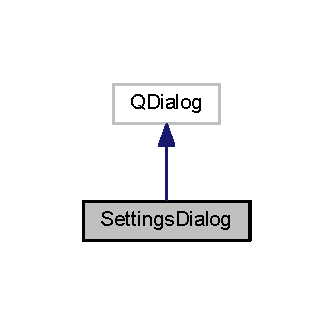
\includegraphics[width=160pt]{class_settings_dialog__inherit__graph}
\end{center}
\end{figure}


Collaboration diagram for Settings\+Dialog\+:
\nopagebreak
\begin{figure}[H]
\begin{center}
\leavevmode
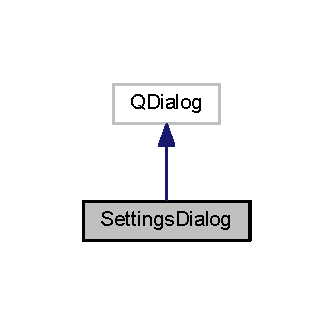
\includegraphics[width=160pt]{class_settings_dialog__coll__graph}
\end{center}
\end{figure}
\subsection*{Classes}
\begin{DoxyCompactItemize}
\item 
struct \hyperlink{struct_settings_dialog_1_1_settings}{Settings}
\end{DoxyCompactItemize}
\subsection*{Public Member Functions}
\begin{DoxyCompactItemize}
\item 
\hyperlink{class_settings_dialog_a9933956b777b2c0451e9119581cc22fb}{Settings\+Dialog} (Q\+Widget $\ast$parent=0)
\item 
\hyperlink{class_settings_dialog_ac48f54d4472902be0a3845a69167f068}{$\sim$\+Settings\+Dialog} ()
\item 
\hyperlink{struct_settings_dialog_1_1_settings}{Settings} \hyperlink{class_settings_dialog_afeb533d711d0392b9856c63b40b65ad7}{settings} () const 
\end{DoxyCompactItemize}


\subsection{Detailed Description}


Definition at line 21 of file settingsdialog.\+h.



\subsection{Constructor \& Destructor Documentation}
\hypertarget{class_settings_dialog_a9933956b777b2c0451e9119581cc22fb}{}\index{Settings\+Dialog@{Settings\+Dialog}!Settings\+Dialog@{Settings\+Dialog}}
\index{Settings\+Dialog@{Settings\+Dialog}!Settings\+Dialog@{Settings\+Dialog}}
\subsubsection[{Settings\+Dialog(\+Q\+Widget $\ast$parent=0)}]{\setlength{\rightskip}{0pt plus 5cm}Settings\+Dialog\+::\+Settings\+Dialog (
\begin{DoxyParamCaption}
\item[{Q\+Widget $\ast$}]{parent = {\ttfamily 0}}
\end{DoxyParamCaption}
)\hspace{0.3cm}{\ttfamily [explicit]}}\label{class_settings_dialog_a9933956b777b2c0451e9119581cc22fb}


Definition at line 12 of file settingsdialog.\+cpp.

\hypertarget{class_settings_dialog_ac48f54d4472902be0a3845a69167f068}{}\index{Settings\+Dialog@{Settings\+Dialog}!````~Settings\+Dialog@{$\sim$\+Settings\+Dialog}}
\index{````~Settings\+Dialog@{$\sim$\+Settings\+Dialog}!Settings\+Dialog@{Settings\+Dialog}}
\subsubsection[{$\sim$\+Settings\+Dialog()}]{\setlength{\rightskip}{0pt plus 5cm}Settings\+Dialog\+::$\sim$\+Settings\+Dialog (
\begin{DoxyParamCaption}
{}
\end{DoxyParamCaption}
)}\label{class_settings_dialog_ac48f54d4472902be0a3845a69167f068}


Definition at line 37 of file settingsdialog.\+cpp.



\subsection{Member Function Documentation}
\hypertarget{class_settings_dialog_afeb533d711d0392b9856c63b40b65ad7}{}\index{Settings\+Dialog@{Settings\+Dialog}!settings@{settings}}
\index{settings@{settings}!Settings\+Dialog@{Settings\+Dialog}}
\subsubsection[{settings() const }]{\setlength{\rightskip}{0pt plus 5cm}{\bf Settings\+Dialog\+::\+Settings} Settings\+Dialog\+::settings (
\begin{DoxyParamCaption}
{}
\end{DoxyParamCaption}
) const}\label{class_settings_dialog_afeb533d711d0392b9856c63b40b65ad7}


Definition at line 42 of file settingsdialog.\+cpp.



The documentation for this class was generated from the following files\+:\begin{DoxyCompactItemize}
\item 
\hyperlink{settingsdialog_8h}{settingsdialog.\+h}\item 
\hyperlink{settingsdialog_8cpp}{settingsdialog.\+cpp}\end{DoxyCompactItemize}

\chapter{File Documentation}
\hypertarget{custom__scene_8cpp}{}\section{custom\+\_\+scene.\+cpp File Reference}
\label{custom__scene_8cpp}\index{custom\+\_\+scene.\+cpp@{custom\+\_\+scene.\+cpp}}
{\ttfamily \#include \char`\"{}custom\+\_\+scene.\+h\char`\"{}}\\*
Include dependency graph for custom\+\_\+scene.\+cpp\+:
\nopagebreak
\begin{figure}[H]
\begin{center}
\leavevmode
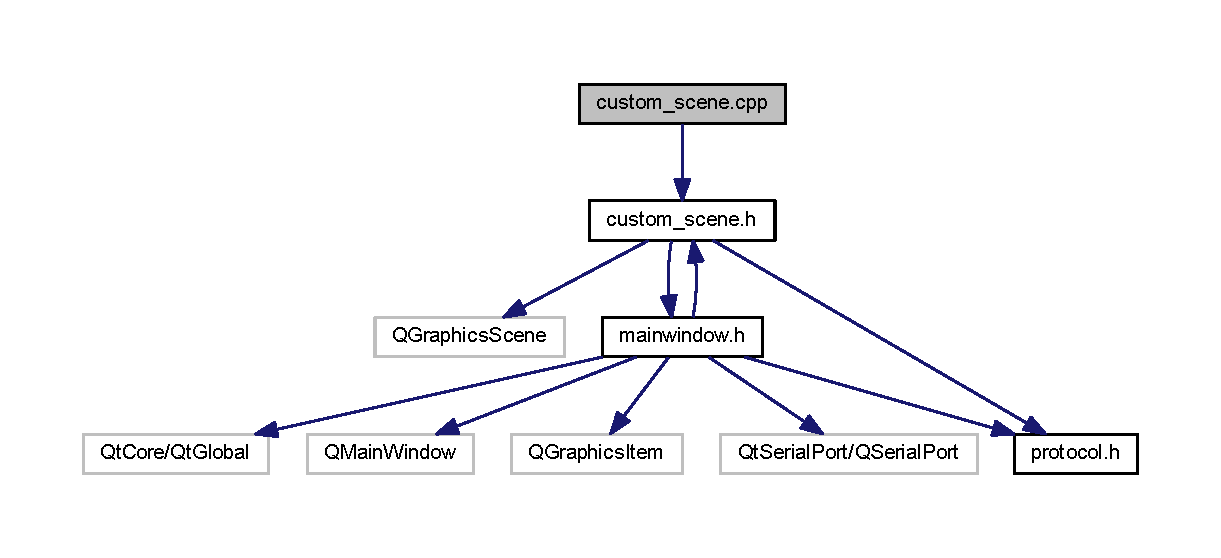
\includegraphics[width=350pt]{custom__scene_8cpp__incl}
\end{center}
\end{figure}

\hypertarget{custom__scene_8h}{}\section{custom\+\_\+scene.\+h File Reference}
\label{custom__scene_8h}\index{custom\+\_\+scene.\+h@{custom\+\_\+scene.\+h}}
{\ttfamily \#include $<$Q\+Graphics\+Scene$>$}\\*
{\ttfamily \#include \char`\"{}mainwindow.\+h\char`\"{}}\\*
{\ttfamily \#include \char`\"{}protocol.\+h\char`\"{}}\\*
Include dependency graph for custom\+\_\+scene.\+h\+:
\nopagebreak
\begin{figure}[H]
\begin{center}
\leavevmode
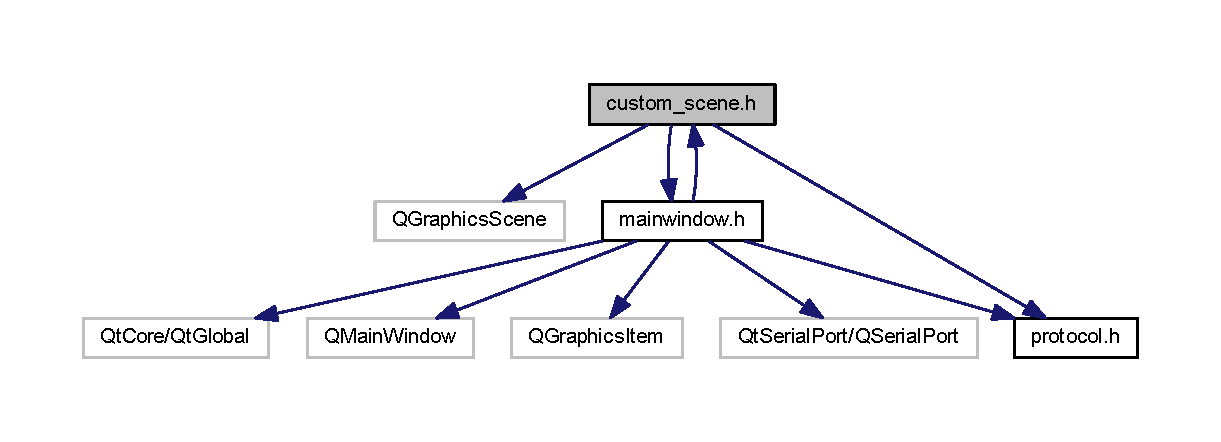
\includegraphics[width=350pt]{custom__scene_8h__incl}
\end{center}
\end{figure}
This graph shows which files directly or indirectly include this file\+:
\nopagebreak
\begin{figure}[H]
\begin{center}
\leavevmode
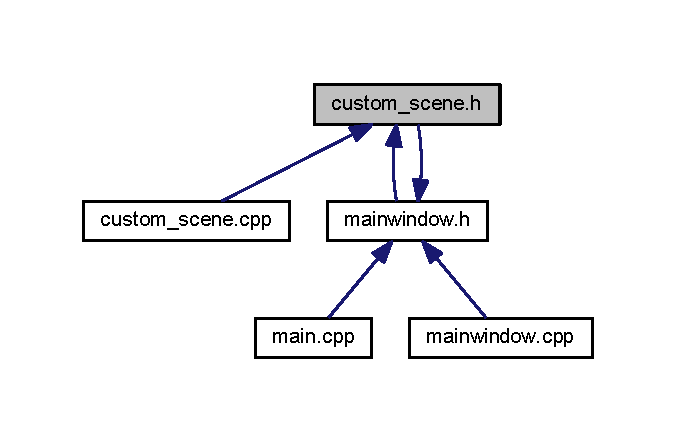
\includegraphics[width=325pt]{custom__scene_8h__dep__incl}
\end{center}
\end{figure}
\subsection*{Classes}
\begin{DoxyCompactItemize}
\item 
class \hyperlink{classcustom__scene}{custom\+\_\+scene}
\end{DoxyCompactItemize}

\hypertarget{_r_e_a_d_m_e_8md}{}\section{doc/\+R\+E\+A\+D\+M\+E.md File Reference}
\label{_r_e_a_d_m_e_8md}\index{doc/\+R\+E\+A\+D\+M\+E.\+md@{doc/\+R\+E\+A\+D\+M\+E.\+md}}

\hypertarget{main_8cpp}{}\section{main.\+cpp File Reference}
\label{main_8cpp}\index{main.\+cpp@{main.\+cpp}}
{\ttfamily \#include $<$Q\+Application$>$}\\*
{\ttfamily \#include \char`\"{}mainwindow.\+h\char`\"{}}\\*
Include dependency graph for main.\+cpp\+:
\nopagebreak
\begin{figure}[H]
\begin{center}
\leavevmode
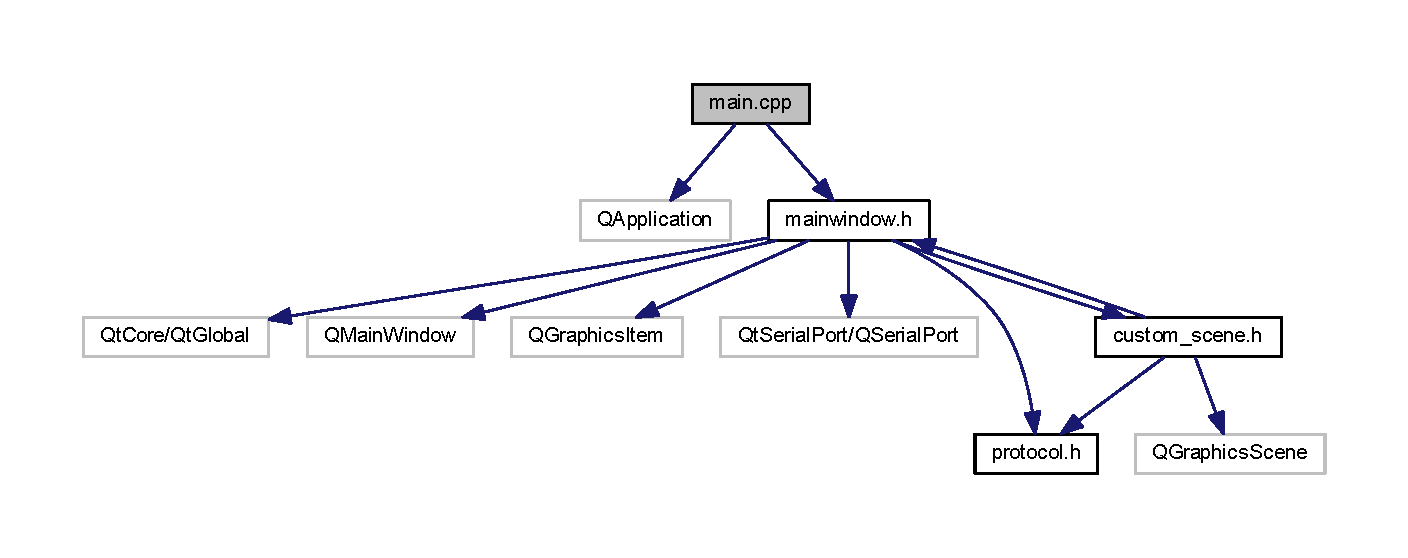
\includegraphics[width=350pt]{main_8cpp__incl}
\end{center}
\end{figure}
\subsection*{Functions}
\begin{DoxyCompactItemize}
\item 
int \hyperlink{main_8cpp_a0ddf1224851353fc92bfbff6f499fa97}{main} (int argc, char $\ast$argv\mbox{[}$\,$\mbox{]})
\end{DoxyCompactItemize}


\subsection{Function Documentation}
\hypertarget{main_8cpp_a0ddf1224851353fc92bfbff6f499fa97}{}\index{main.\+cpp@{main.\+cpp}!main@{main}}
\index{main@{main}!main.\+cpp@{main.\+cpp}}
\subsubsection[{main(int argc, char $\ast$argv[])}]{\setlength{\rightskip}{0pt plus 5cm}int main (
\begin{DoxyParamCaption}
\item[{int}]{argc, }
\item[{char $\ast$}]{argv\mbox{[}$\,$\mbox{]}}
\end{DoxyParamCaption}
)}\label{main_8cpp_a0ddf1224851353fc92bfbff6f499fa97}


Definition at line 5 of file main.\+cpp.


\hypertarget{mainwindow_8cpp}{}\section{mainwindow.\+cpp File Reference}
\label{mainwindow_8cpp}\index{mainwindow.\+cpp@{mainwindow.\+cpp}}
{\ttfamily \#include \char`\"{}mainwindow.\+h\char`\"{}}\\*
{\ttfamily \#include \char`\"{}ui\+\_\+mainwindow.\+h\char`\"{}}\\*
{\ttfamily \#include \char`\"{}settingsdialog.\+h\char`\"{}}\\*
{\ttfamily \#include $<$Q\+Message\+Box$>$}\\*
{\ttfamily \#include $<$Q\+Label$>$}\\*
{\ttfamily \#include $<$Qt\+Serial\+Port/\+Q\+Serial\+Port$>$}\\*
Include dependency graph for mainwindow.\+cpp\+:
\nopagebreak
\begin{figure}[H]
\begin{center}
\leavevmode
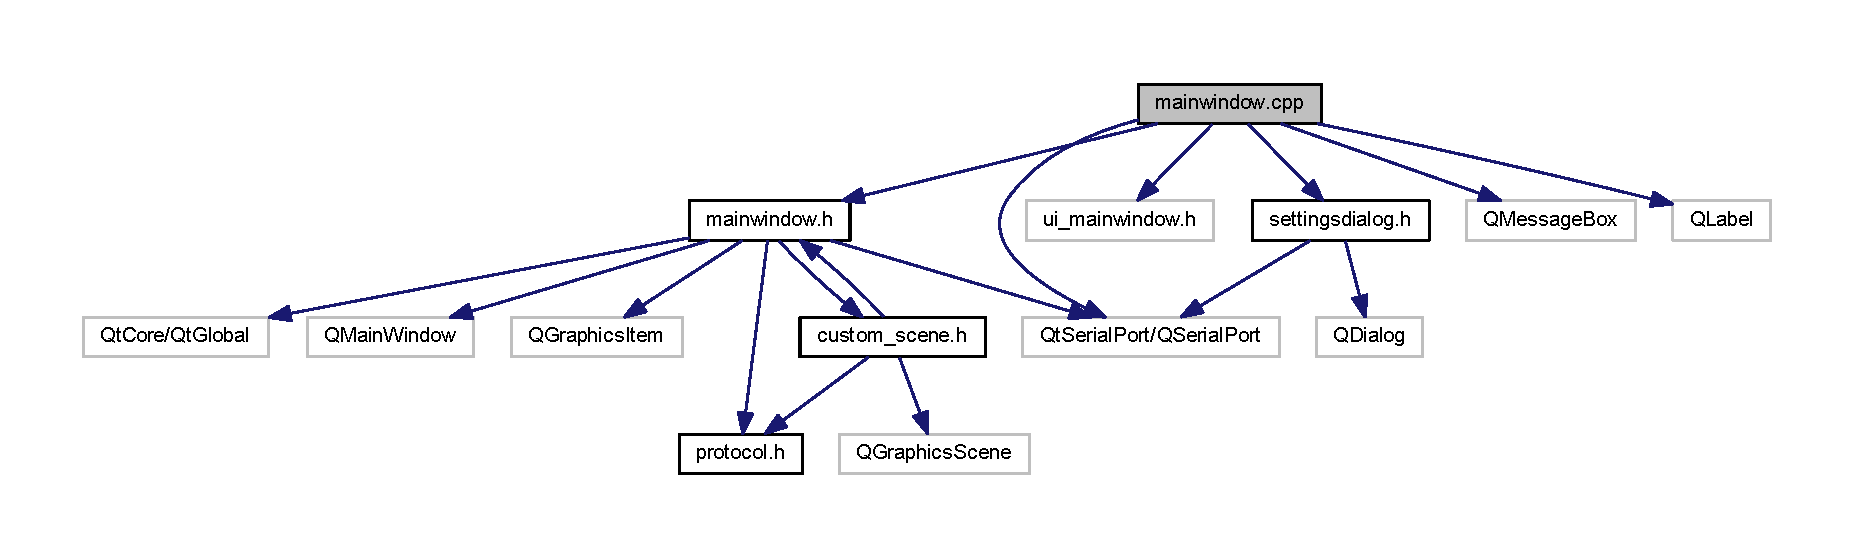
\includegraphics[width=350pt]{mainwindow_8cpp__incl}
\end{center}
\end{figure}

\hypertarget{mainwindow_8h}{}\section{mainwindow.\+h File Reference}
\label{mainwindow_8h}\index{mainwindow.\+h@{mainwindow.\+h}}
{\ttfamily \#include $<$Qt\+Core/\+Qt\+Global$>$}\\*
{\ttfamily \#include $<$Q\+Main\+Window$>$}\\*
{\ttfamily \#include $<$Q\+Graphics\+Item$>$}\\*
{\ttfamily \#include $<$Qt\+Serial\+Port/\+Q\+Serial\+Port$>$}\\*
{\ttfamily \#include \char`\"{}protocol.\+h\char`\"{}}\\*
{\ttfamily \#include \char`\"{}custom\+\_\+scene.\+h\char`\"{}}\\*
Include dependency graph for mainwindow.\+h\+:
\nopagebreak
\begin{figure}[H]
\begin{center}
\leavevmode
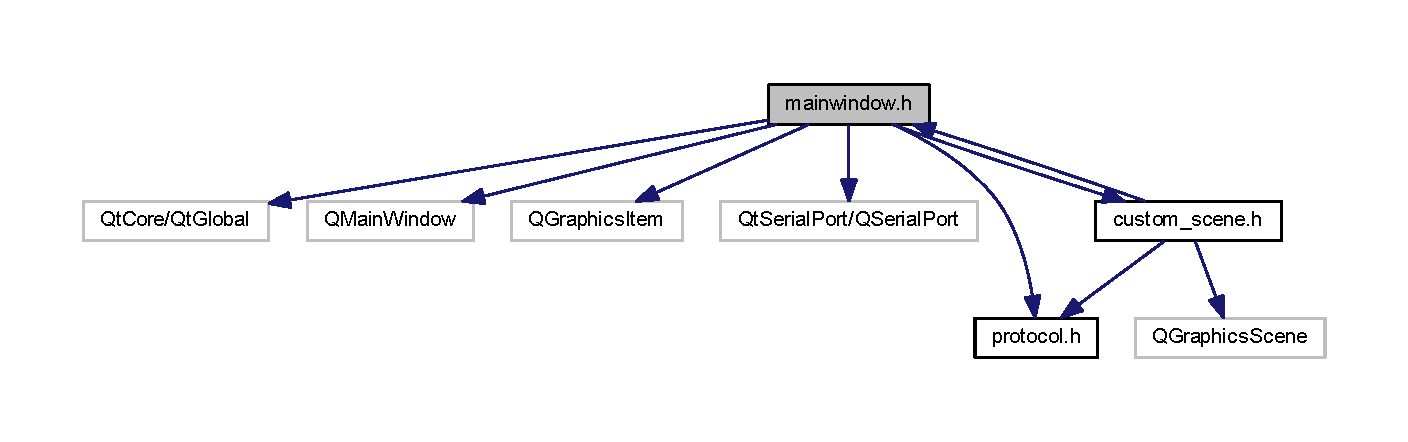
\includegraphics[width=350pt]{mainwindow_8h__incl}
\end{center}
\end{figure}
This graph shows which files directly or indirectly include this file\+:
\nopagebreak
\begin{figure}[H]
\begin{center}
\leavevmode
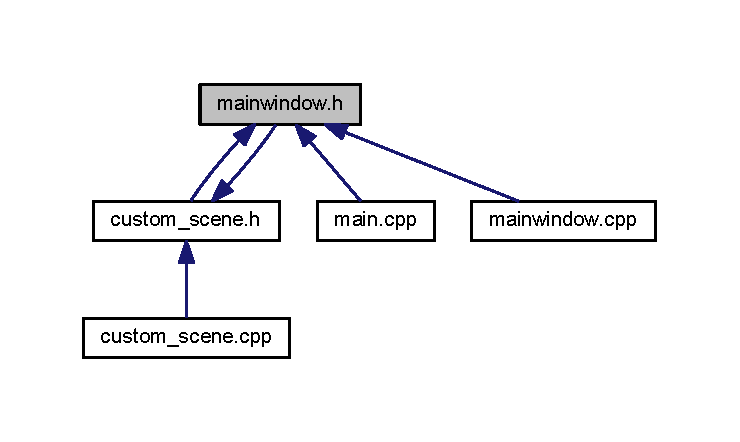
\includegraphics[width=350pt]{mainwindow_8h__dep__incl}
\end{center}
\end{figure}
\subsection*{Classes}
\begin{DoxyCompactItemize}
\item 
class \hyperlink{class_main_window}{Main\+Window}
\end{DoxyCompactItemize}
\subsection*{Namespaces}
\begin{DoxyCompactItemize}
\item 
 \hyperlink{namespace_ui}{Ui}
\end{DoxyCompactItemize}

\hypertarget{protocol_8cpp}{}\section{protocol.\+cpp File Reference}
\label{protocol_8cpp}\index{protocol.\+cpp@{protocol.\+cpp}}
{\ttfamily \#include \char`\"{}protocol.\+h\char`\"{}}\\*
Include dependency graph for protocol.\+cpp\+:
\nopagebreak
\begin{figure}[H]
\begin{center}
\leavevmode
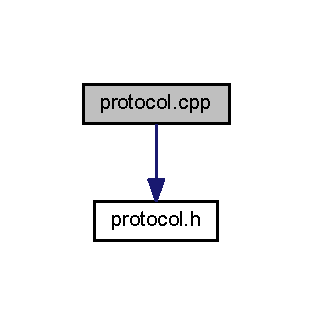
\includegraphics[width=150pt]{protocol_8cpp__incl}
\end{center}
\end{figure}
\subsection*{Functions}
\begin{DoxyCompactItemize}
\item 
unsigned char $\ast$ \hyperlink{protocol_8cpp_a9776eee48cf368cd56f8abf85a993a10}{Apply\+Protocol} (\hyperlink{protocol_8h_ae5051f6f612e6d4218717f733bc50667}{Message} $\ast$msg)
\begin{DoxyCompactList}\small\item\em Both native and Qt implementation. \end{DoxyCompactList}\item 
\hyperlink{protocol_8h_ae5051f6f612e6d4218717f733bc50667}{Message} $\ast$ \hyperlink{protocol_8cpp_ae6d4e4f8050d33a7636d23d1ab67a446}{Read\+Frame} (unsigned char $\ast$frame, unsigned int size)
\begin{DoxyCompactList}\small\item\em Read a frame. \end{DoxyCompactList}\end{DoxyCompactItemize}


\subsection{Function Documentation}
\hypertarget{protocol_8cpp_a9776eee48cf368cd56f8abf85a993a10}{}\index{protocol.\+cpp@{protocol.\+cpp}!Apply\+Protocol@{Apply\+Protocol}}
\index{Apply\+Protocol@{Apply\+Protocol}!protocol.\+cpp@{protocol.\+cpp}}
\subsubsection[{Apply\+Protocol(\+Message $\ast$msg)}]{\setlength{\rightskip}{0pt plus 5cm}unsigned char$\ast$ Apply\+Protocol (
\begin{DoxyParamCaption}
\item[{{\bf Message} $\ast$}]{msg}
\end{DoxyParamCaption}
)}\label{protocol_8cpp_a9776eee48cf368cd56f8abf85a993a10}


Both native and Qt implementation. 

Write a transmitable array. $<$ Apply transmission offset on data 
\begin{DoxyParams}{Parameters}
{\em msg} & Write a transmitable array \\
\hline
\end{DoxyParams}


Definition at line 9 of file protocol.\+cpp.



Here is the caller graph for this function\+:
\nopagebreak
\begin{figure}[H]
\begin{center}
\leavevmode
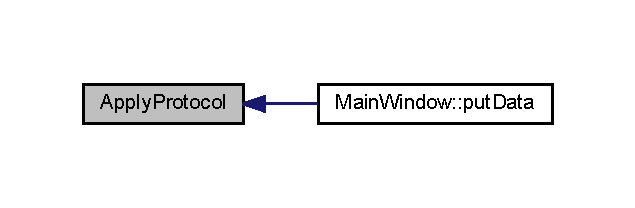
\includegraphics[width=305pt]{protocol_8cpp_a9776eee48cf368cd56f8abf85a993a10_icgraph}
\end{center}
\end{figure}


\hypertarget{protocol_8cpp_ae6d4e4f8050d33a7636d23d1ab67a446}{}\index{protocol.\+cpp@{protocol.\+cpp}!Read\+Frame@{Read\+Frame}}
\index{Read\+Frame@{Read\+Frame}!protocol.\+cpp@{protocol.\+cpp}}
\subsubsection[{Read\+Frame(unsigned char $\ast$frame, unsigned int size)}]{\setlength{\rightskip}{0pt plus 5cm}{\bf Message}$\ast$ Read\+Frame (
\begin{DoxyParamCaption}
\item[{unsigned char $\ast$}]{frame, }
\item[{unsigned int}]{size}
\end{DoxyParamCaption}
)}\label{protocol_8cpp_ae6d4e4f8050d33a7636d23d1ab67a446}


Read a frame. 

$<$ Search for a \char`\"{}start of header\char`\"{} char

$<$ If no header

$<$ If receiving standard data

$<$ Read all data

$<$ If reach end without encountering S\+T\+O\+P\+\_\+\+D\+A\+T\+A and S\+T\+O\+P\+\_\+\+T\+R\+A\+N\+S\+M\+I\+S\+S\+I\+O\+N

$<$ If no data block

$<$ If receiving a N\+A\+C\+K or A\+C\+K 

Definition at line 26 of file protocol.\+cpp.


\hypertarget{protocol_8h}{}\section{protocol.\+h File Reference}
\label{protocol_8h}\index{protocol.\+h@{protocol.\+h}}
This graph shows which files directly or indirectly include this file\+:
\nopagebreak
\begin{figure}[H]
\begin{center}
\leavevmode
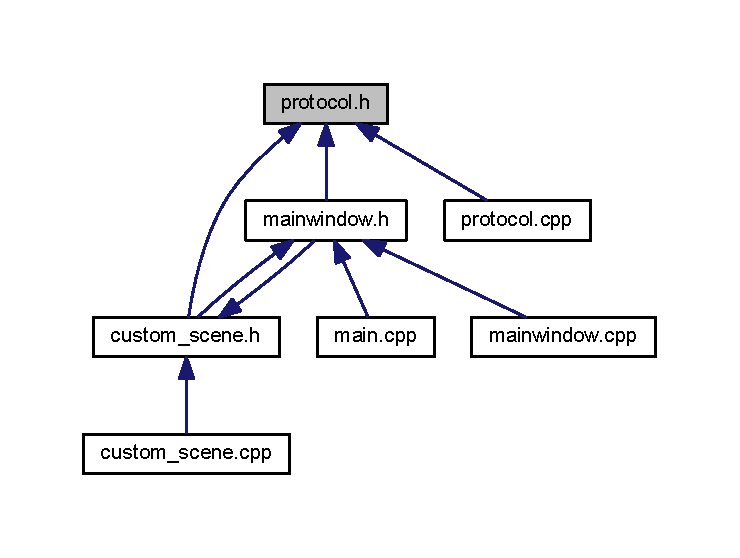
\includegraphics[width=350pt]{protocol_8h__dep__incl}
\end{center}
\end{figure}
\subsection*{Classes}
\begin{DoxyCompactItemize}
\item 
struct \hyperlink{structmessage}{message}
\end{DoxyCompactItemize}
\subsection*{Typedefs}
\begin{DoxyCompactItemize}
\item 
typedef struct \hyperlink{structmessage}{message} \hyperlink{protocol_8h_ae5051f6f612e6d4218717f733bc50667}{Message}
\end{DoxyCompactItemize}
\subsection*{Enumerations}
\begin{DoxyCompactItemize}
\item 
enum \hyperlink{protocol_8h_ad327bde01da3f3f8f71ae03db02572bc}{Protocol} \+: unsigned char \{ \\*
\hyperlink{protocol_8h_ad327bde01da3f3f8f71ae03db02572bcaa67e934c7b9fcd7986f2122cbb316c90}{S\+T\+A\+R\+T\+\_\+\+H\+E\+A\+D\+E\+R} =1, 
\hyperlink{protocol_8h_ad327bde01da3f3f8f71ae03db02572bca9ff6e0136f603bd7b79bf27bf3bcf631}{S\+T\+A\+R\+T\+\_\+\+D\+A\+T\+A} =2, 
\hyperlink{protocol_8h_ad327bde01da3f3f8f71ae03db02572bca32f4638400387174a8f7ec501559ea7e}{S\+T\+O\+P\+\_\+\+D\+A\+T\+A} =3, 
\hyperlink{protocol_8h_ad327bde01da3f3f8f71ae03db02572bcaa9a20b0c7a383cd6aa2742298b10a627}{S\+T\+O\+P\+\_\+\+F\+R\+A\+M\+E} =4, 
\\*
\hyperlink{protocol_8h_ad327bde01da3f3f8f71ae03db02572bca1c986c1141c1160cd172cbde2ce18166}{N\+A\+C\+K} =21, 
\hyperlink{protocol_8h_ad327bde01da3f3f8f71ae03db02572bca41246e9c8691b7e33bc79b345e06b48e}{A\+C\+K} =6, 
\hyperlink{protocol_8h_ad327bde01da3f3f8f71ae03db02572bcadf9227ae7f4f43eb87b8648334d70486}{M\+O\+D\+E\+\_\+\+A\+U\+T\+O} =19, 
\hyperlink{protocol_8h_ad327bde01da3f3f8f71ae03db02572bcaa56e5070fb0450a65a216279d93fe934}{M\+O\+D\+E\+\_\+\+T\+R\+A\+C\+K\+I\+N\+G} =20, 
\\*
\hyperlink{protocol_8h_ad327bde01da3f3f8f71ae03db02572bca672168f72a883ddaff3605bb9b3e696b}{D\+A\+T\+A\+\_\+\+S\+E\+P\+A\+R\+A\+T\+O\+R} =29, 
\hyperlink{protocol_8h_ad327bde01da3f3f8f71ae03db02572bcad9ff273a12ff18b3e1b900080aadd1ea}{C\+U\+B\+E} =40, 
\hyperlink{protocol_8h_ad327bde01da3f3f8f71ae03db02572bca59c6b7739f239fb18fe5c81692358893}{E\+L\+L\+I\+P\+S\+E} =41, 
\hyperlink{protocol_8h_ad327bde01da3f3f8f71ae03db02572bca2fd33892864d1c342d3bead2f2d9ad56}{T\+R\+I\+A\+N\+G\+L\+E} =42, 
\\*
\hyperlink{protocol_8h_ad327bde01da3f3f8f71ae03db02572bca2f68568c4f2b54aa1007c249ff0d75ed}{P\+O\+S\+I\+T\+I\+O\+N\+\_\+\+L\+O\+W\+E\+R\+\_\+\+L\+I\+M\+I\+T} =0, 
\hyperlink{protocol_8h_ad327bde01da3f3f8f71ae03db02572bca9aa52b99370653232b3c1482f2732b6c}{P\+O\+S\+I\+T\+I\+O\+N\+\_\+\+U\+P\+P\+E\+R\+\_\+\+L\+I\+M\+I\+T} =180, 
\hyperlink{protocol_8h_ad327bde01da3f3f8f71ae03db02572bca831aca8dcd0e3a3fdb63b9c87ea7a412}{T\+R\+A\+N\+S\+M\+I\+S\+S\+I\+O\+N\+\_\+\+O\+F\+F\+S\+E\+T} =32
 \}
\item 
enum \hyperlink{protocol_8h_a001559174c1105d69e7939fd2d1dcebc}{Error\+Code} \+: unsigned char \{ \hyperlink{protocol_8h_a001559174c1105d69e7939fd2d1dcebca86d8adc4c0423a641dc4cdeaa20bbb74}{N\+O\+\_\+\+F\+R\+A\+M\+E} =0, 
\hyperlink{protocol_8h_a001559174c1105d69e7939fd2d1dcebca5ebb369e927979b7c092415b36f807db}{U\+N\+T\+E\+R\+M\+I\+N\+A\+T\+E\+D\+\_\+\+F\+R\+A\+M\+E} =1
 \}
\end{DoxyCompactItemize}
\subsection*{Functions}
\begin{DoxyCompactItemize}
\item 
unsigned char $\ast$ \hyperlink{protocol_8h_a9776eee48cf368cd56f8abf85a993a10}{Apply\+Protocol} (\hyperlink{protocol_8h_ae5051f6f612e6d4218717f733bc50667}{Message} $\ast$msg)
\begin{DoxyCompactList}\small\item\em Write a transmitable array. \end{DoxyCompactList}\item 
\hyperlink{protocol_8h_ae5051f6f612e6d4218717f733bc50667}{Message} $\ast$ \hyperlink{protocol_8h_ae6d4e4f8050d33a7636d23d1ab67a446}{Read\+Frame} (unsigned char $\ast$frame, unsigned int size)
\begin{DoxyCompactList}\small\item\em Read a frame. \end{DoxyCompactList}\end{DoxyCompactItemize}


\subsection{Typedef Documentation}
\hypertarget{protocol_8h_ae5051f6f612e6d4218717f733bc50667}{}\index{protocol.\+h@{protocol.\+h}!Message@{Message}}
\index{Message@{Message}!protocol.\+h@{protocol.\+h}}
\subsubsection[{Message}]{\setlength{\rightskip}{0pt plus 5cm}typedef struct {\bf message}  {\bf Message}}\label{protocol_8h_ae5051f6f612e6d4218717f733bc50667}
Structure used by functions to read and write according to the protocol. You can interact with functions only through this structure. No verification is done on the struct, so be carefull when you assign data. Otherwise, you\textquotesingle{}ll send corrupted packet and the board will answer N\+A\+C\+K. 

\subsection{Enumeration Type Documentation}
\hypertarget{protocol_8h_a001559174c1105d69e7939fd2d1dcebc}{}\index{protocol.\+h@{protocol.\+h}!Error\+Code@{Error\+Code}}
\index{Error\+Code@{Error\+Code}!protocol.\+h@{protocol.\+h}}
\subsubsection[{Error\+Code}]{\setlength{\rightskip}{0pt plus 5cm}enum {\bf Error\+Code} \+: unsigned char}\label{protocol_8h_a001559174c1105d69e7939fd2d1dcebc}
\begin{Desc}
\item[Enumerator]\par
\begin{description}
\index{N\+O\+\_\+\+F\+R\+A\+M\+E@{N\+O\+\_\+\+F\+R\+A\+M\+E}!protocol.\+h@{protocol.\+h}}\index{protocol.\+h@{protocol.\+h}!N\+O\+\_\+\+F\+R\+A\+M\+E@{N\+O\+\_\+\+F\+R\+A\+M\+E}}\item[{\em 
\hypertarget{protocol_8h_a001559174c1105d69e7939fd2d1dcebca86d8adc4c0423a641dc4cdeaa20bbb74}{}N\+O\+\_\+\+F\+R\+A\+M\+E\label{protocol_8h_a001559174c1105d69e7939fd2d1dcebca86d8adc4c0423a641dc4cdeaa20bbb74}
}]\index{U\+N\+T\+E\+R\+M\+I\+N\+A\+T\+E\+D\+\_\+\+F\+R\+A\+M\+E@{U\+N\+T\+E\+R\+M\+I\+N\+A\+T\+E\+D\+\_\+\+F\+R\+A\+M\+E}!protocol.\+h@{protocol.\+h}}\index{protocol.\+h@{protocol.\+h}!U\+N\+T\+E\+R\+M\+I\+N\+A\+T\+E\+D\+\_\+\+F\+R\+A\+M\+E@{U\+N\+T\+E\+R\+M\+I\+N\+A\+T\+E\+D\+\_\+\+F\+R\+A\+M\+E}}\item[{\em 
\hypertarget{protocol_8h_a001559174c1105d69e7939fd2d1dcebca5ebb369e927979b7c092415b36f807db}{}U\+N\+T\+E\+R\+M\+I\+N\+A\+T\+E\+D\+\_\+\+F\+R\+A\+M\+E\label{protocol_8h_a001559174c1105d69e7939fd2d1dcebca5ebb369e927979b7c092415b36f807db}
}]\end{description}
\end{Desc}


Definition at line 26 of file protocol.\+h.

\hypertarget{protocol_8h_ad327bde01da3f3f8f71ae03db02572bc}{}\index{protocol.\+h@{protocol.\+h}!Protocol@{Protocol}}
\index{Protocol@{Protocol}!protocol.\+h@{protocol.\+h}}
\subsubsection[{Protocol}]{\setlength{\rightskip}{0pt plus 5cm}enum {\bf Protocol} \+: unsigned char}\label{protocol_8h_ad327bde01da3f3f8f71ae03db02572bc}
\begin{DoxyAuthor}{Author}
Quentin Berdal 
\end{DoxyAuthor}
\begin{Desc}
\item[Enumerator]\par
\begin{description}
\index{S\+T\+A\+R\+T\+\_\+\+H\+E\+A\+D\+E\+R@{S\+T\+A\+R\+T\+\_\+\+H\+E\+A\+D\+E\+R}!protocol.\+h@{protocol.\+h}}\index{protocol.\+h@{protocol.\+h}!S\+T\+A\+R\+T\+\_\+\+H\+E\+A\+D\+E\+R@{S\+T\+A\+R\+T\+\_\+\+H\+E\+A\+D\+E\+R}}\item[{\em 
\hypertarget{protocol_8h_ad327bde01da3f3f8f71ae03db02572bcaa67e934c7b9fcd7986f2122cbb316c90}{}S\+T\+A\+R\+T\+\_\+\+H\+E\+A\+D\+E\+R\label{protocol_8h_ad327bde01da3f3f8f71ae03db02572bcaa67e934c7b9fcd7986f2122cbb316c90}
}]\index{S\+T\+A\+R\+T\+\_\+\+D\+A\+T\+A@{S\+T\+A\+R\+T\+\_\+\+D\+A\+T\+A}!protocol.\+h@{protocol.\+h}}\index{protocol.\+h@{protocol.\+h}!S\+T\+A\+R\+T\+\_\+\+D\+A\+T\+A@{S\+T\+A\+R\+T\+\_\+\+D\+A\+T\+A}}\item[{\em 
\hypertarget{protocol_8h_ad327bde01da3f3f8f71ae03db02572bca9ff6e0136f603bd7b79bf27bf3bcf631}{}S\+T\+A\+R\+T\+\_\+\+D\+A\+T\+A\label{protocol_8h_ad327bde01da3f3f8f71ae03db02572bca9ff6e0136f603bd7b79bf27bf3bcf631}
}]\index{S\+T\+O\+P\+\_\+\+D\+A\+T\+A@{S\+T\+O\+P\+\_\+\+D\+A\+T\+A}!protocol.\+h@{protocol.\+h}}\index{protocol.\+h@{protocol.\+h}!S\+T\+O\+P\+\_\+\+D\+A\+T\+A@{S\+T\+O\+P\+\_\+\+D\+A\+T\+A}}\item[{\em 
\hypertarget{protocol_8h_ad327bde01da3f3f8f71ae03db02572bca32f4638400387174a8f7ec501559ea7e}{}S\+T\+O\+P\+\_\+\+D\+A\+T\+A\label{protocol_8h_ad327bde01da3f3f8f71ae03db02572bca32f4638400387174a8f7ec501559ea7e}
}]\index{S\+T\+O\+P\+\_\+\+F\+R\+A\+M\+E@{S\+T\+O\+P\+\_\+\+F\+R\+A\+M\+E}!protocol.\+h@{protocol.\+h}}\index{protocol.\+h@{protocol.\+h}!S\+T\+O\+P\+\_\+\+F\+R\+A\+M\+E@{S\+T\+O\+P\+\_\+\+F\+R\+A\+M\+E}}\item[{\em 
\hypertarget{protocol_8h_ad327bde01da3f3f8f71ae03db02572bcaa9a20b0c7a383cd6aa2742298b10a627}{}S\+T\+O\+P\+\_\+\+F\+R\+A\+M\+E\label{protocol_8h_ad327bde01da3f3f8f71ae03db02572bcaa9a20b0c7a383cd6aa2742298b10a627}
}]\index{N\+A\+C\+K@{N\+A\+C\+K}!protocol.\+h@{protocol.\+h}}\index{protocol.\+h@{protocol.\+h}!N\+A\+C\+K@{N\+A\+C\+K}}\item[{\em 
\hypertarget{protocol_8h_ad327bde01da3f3f8f71ae03db02572bca1c986c1141c1160cd172cbde2ce18166}{}N\+A\+C\+K\label{protocol_8h_ad327bde01da3f3f8f71ae03db02572bca1c986c1141c1160cd172cbde2ce18166}
}]\index{A\+C\+K@{A\+C\+K}!protocol.\+h@{protocol.\+h}}\index{protocol.\+h@{protocol.\+h}!A\+C\+K@{A\+C\+K}}\item[{\em 
\hypertarget{protocol_8h_ad327bde01da3f3f8f71ae03db02572bca41246e9c8691b7e33bc79b345e06b48e}{}A\+C\+K\label{protocol_8h_ad327bde01da3f3f8f71ae03db02572bca41246e9c8691b7e33bc79b345e06b48e}
}]\index{M\+O\+D\+E\+\_\+\+A\+U\+T\+O@{M\+O\+D\+E\+\_\+\+A\+U\+T\+O}!protocol.\+h@{protocol.\+h}}\index{protocol.\+h@{protocol.\+h}!M\+O\+D\+E\+\_\+\+A\+U\+T\+O@{M\+O\+D\+E\+\_\+\+A\+U\+T\+O}}\item[{\em 
\hypertarget{protocol_8h_ad327bde01da3f3f8f71ae03db02572bcadf9227ae7f4f43eb87b8648334d70486}{}M\+O\+D\+E\+\_\+\+A\+U\+T\+O\label{protocol_8h_ad327bde01da3f3f8f71ae03db02572bcadf9227ae7f4f43eb87b8648334d70486}
}]\index{M\+O\+D\+E\+\_\+\+T\+R\+A\+C\+K\+I\+N\+G@{M\+O\+D\+E\+\_\+\+T\+R\+A\+C\+K\+I\+N\+G}!protocol.\+h@{protocol.\+h}}\index{protocol.\+h@{protocol.\+h}!M\+O\+D\+E\+\_\+\+T\+R\+A\+C\+K\+I\+N\+G@{M\+O\+D\+E\+\_\+\+T\+R\+A\+C\+K\+I\+N\+G}}\item[{\em 
\hypertarget{protocol_8h_ad327bde01da3f3f8f71ae03db02572bcaa56e5070fb0450a65a216279d93fe934}{}M\+O\+D\+E\+\_\+\+T\+R\+A\+C\+K\+I\+N\+G\label{protocol_8h_ad327bde01da3f3f8f71ae03db02572bcaa56e5070fb0450a65a216279d93fe934}
}]\index{D\+A\+T\+A\+\_\+\+S\+E\+P\+A\+R\+A\+T\+O\+R@{D\+A\+T\+A\+\_\+\+S\+E\+P\+A\+R\+A\+T\+O\+R}!protocol.\+h@{protocol.\+h}}\index{protocol.\+h@{protocol.\+h}!D\+A\+T\+A\+\_\+\+S\+E\+P\+A\+R\+A\+T\+O\+R@{D\+A\+T\+A\+\_\+\+S\+E\+P\+A\+R\+A\+T\+O\+R}}\item[{\em 
\hypertarget{protocol_8h_ad327bde01da3f3f8f71ae03db02572bca672168f72a883ddaff3605bb9b3e696b}{}D\+A\+T\+A\+\_\+\+S\+E\+P\+A\+R\+A\+T\+O\+R\label{protocol_8h_ad327bde01da3f3f8f71ae03db02572bca672168f72a883ddaff3605bb9b3e696b}
}]\index{C\+U\+B\+E@{C\+U\+B\+E}!protocol.\+h@{protocol.\+h}}\index{protocol.\+h@{protocol.\+h}!C\+U\+B\+E@{C\+U\+B\+E}}\item[{\em 
\hypertarget{protocol_8h_ad327bde01da3f3f8f71ae03db02572bcad9ff273a12ff18b3e1b900080aadd1ea}{}C\+U\+B\+E\label{protocol_8h_ad327bde01da3f3f8f71ae03db02572bcad9ff273a12ff18b3e1b900080aadd1ea}
}]\index{E\+L\+L\+I\+P\+S\+E@{E\+L\+L\+I\+P\+S\+E}!protocol.\+h@{protocol.\+h}}\index{protocol.\+h@{protocol.\+h}!E\+L\+L\+I\+P\+S\+E@{E\+L\+L\+I\+P\+S\+E}}\item[{\em 
\hypertarget{protocol_8h_ad327bde01da3f3f8f71ae03db02572bca59c6b7739f239fb18fe5c81692358893}{}E\+L\+L\+I\+P\+S\+E\label{protocol_8h_ad327bde01da3f3f8f71ae03db02572bca59c6b7739f239fb18fe5c81692358893}
}]\index{T\+R\+I\+A\+N\+G\+L\+E@{T\+R\+I\+A\+N\+G\+L\+E}!protocol.\+h@{protocol.\+h}}\index{protocol.\+h@{protocol.\+h}!T\+R\+I\+A\+N\+G\+L\+E@{T\+R\+I\+A\+N\+G\+L\+E}}\item[{\em 
\hypertarget{protocol_8h_ad327bde01da3f3f8f71ae03db02572bca2fd33892864d1c342d3bead2f2d9ad56}{}T\+R\+I\+A\+N\+G\+L\+E\label{protocol_8h_ad327bde01da3f3f8f71ae03db02572bca2fd33892864d1c342d3bead2f2d9ad56}
}]\index{P\+O\+S\+I\+T\+I\+O\+N\+\_\+\+L\+O\+W\+E\+R\+\_\+\+L\+I\+M\+I\+T@{P\+O\+S\+I\+T\+I\+O\+N\+\_\+\+L\+O\+W\+E\+R\+\_\+\+L\+I\+M\+I\+T}!protocol.\+h@{protocol.\+h}}\index{protocol.\+h@{protocol.\+h}!P\+O\+S\+I\+T\+I\+O\+N\+\_\+\+L\+O\+W\+E\+R\+\_\+\+L\+I\+M\+I\+T@{P\+O\+S\+I\+T\+I\+O\+N\+\_\+\+L\+O\+W\+E\+R\+\_\+\+L\+I\+M\+I\+T}}\item[{\em 
\hypertarget{protocol_8h_ad327bde01da3f3f8f71ae03db02572bca2f68568c4f2b54aa1007c249ff0d75ed}{}P\+O\+S\+I\+T\+I\+O\+N\+\_\+\+L\+O\+W\+E\+R\+\_\+\+L\+I\+M\+I\+T\label{protocol_8h_ad327bde01da3f3f8f71ae03db02572bca2f68568c4f2b54aa1007c249ff0d75ed}
}]\index{P\+O\+S\+I\+T\+I\+O\+N\+\_\+\+U\+P\+P\+E\+R\+\_\+\+L\+I\+M\+I\+T@{P\+O\+S\+I\+T\+I\+O\+N\+\_\+\+U\+P\+P\+E\+R\+\_\+\+L\+I\+M\+I\+T}!protocol.\+h@{protocol.\+h}}\index{protocol.\+h@{protocol.\+h}!P\+O\+S\+I\+T\+I\+O\+N\+\_\+\+U\+P\+P\+E\+R\+\_\+\+L\+I\+M\+I\+T@{P\+O\+S\+I\+T\+I\+O\+N\+\_\+\+U\+P\+P\+E\+R\+\_\+\+L\+I\+M\+I\+T}}\item[{\em 
\hypertarget{protocol_8h_ad327bde01da3f3f8f71ae03db02572bca9aa52b99370653232b3c1482f2732b6c}{}P\+O\+S\+I\+T\+I\+O\+N\+\_\+\+U\+P\+P\+E\+R\+\_\+\+L\+I\+M\+I\+T\label{protocol_8h_ad327bde01da3f3f8f71ae03db02572bca9aa52b99370653232b3c1482f2732b6c}
}]\index{T\+R\+A\+N\+S\+M\+I\+S\+S\+I\+O\+N\+\_\+\+O\+F\+F\+S\+E\+T@{T\+R\+A\+N\+S\+M\+I\+S\+S\+I\+O\+N\+\_\+\+O\+F\+F\+S\+E\+T}!protocol.\+h@{protocol.\+h}}\index{protocol.\+h@{protocol.\+h}!T\+R\+A\+N\+S\+M\+I\+S\+S\+I\+O\+N\+\_\+\+O\+F\+F\+S\+E\+T@{T\+R\+A\+N\+S\+M\+I\+S\+S\+I\+O\+N\+\_\+\+O\+F\+F\+S\+E\+T}}\item[{\em 
\hypertarget{protocol_8h_ad327bde01da3f3f8f71ae03db02572bca831aca8dcd0e3a3fdb63b9c87ea7a412}{}T\+R\+A\+N\+S\+M\+I\+S\+S\+I\+O\+N\+\_\+\+O\+F\+F\+S\+E\+T\label{protocol_8h_ad327bde01da3f3f8f71ae03db02572bca831aca8dcd0e3a3fdb63b9c87ea7a412}
}]\end{description}
\end{Desc}


Definition at line 7 of file protocol.\+h.



\subsection{Function Documentation}
\hypertarget{protocol_8h_a9776eee48cf368cd56f8abf85a993a10}{}\index{protocol.\+h@{protocol.\+h}!Apply\+Protocol@{Apply\+Protocol}}
\index{Apply\+Protocol@{Apply\+Protocol}!protocol.\+h@{protocol.\+h}}
\subsubsection[{Apply\+Protocol(\+Message $\ast$msg)}]{\setlength{\rightskip}{0pt plus 5cm}unsigned char$\ast$ Apply\+Protocol (
\begin{DoxyParamCaption}
\item[{{\bf Message} $\ast$}]{msg}
\end{DoxyParamCaption}
)}\label{protocol_8h_a9776eee48cf368cd56f8abf85a993a10}


Write a transmitable array. 

Write a transmitable array. $<$ Apply transmission offset on data 
\begin{DoxyParams}{Parameters}
{\em msg} & Write a transmitable array \\
\hline
\end{DoxyParams}


Definition at line 9 of file protocol.\+cpp.



Here is the caller graph for this function\+:
\nopagebreak
\begin{figure}[H]
\begin{center}
\leavevmode
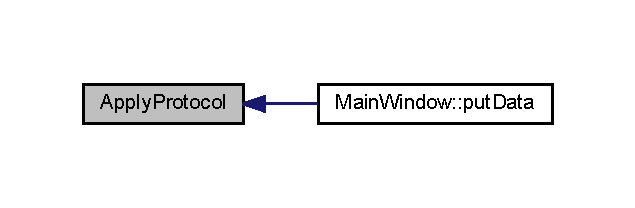
\includegraphics[width=305pt]{protocol_8h_a9776eee48cf368cd56f8abf85a993a10_icgraph}
\end{center}
\end{figure}


\hypertarget{protocol_8h_ae6d4e4f8050d33a7636d23d1ab67a446}{}\index{protocol.\+h@{protocol.\+h}!Read\+Frame@{Read\+Frame}}
\index{Read\+Frame@{Read\+Frame}!protocol.\+h@{protocol.\+h}}
\subsubsection[{Read\+Frame(unsigned char $\ast$frame, unsigned int size)}]{\setlength{\rightskip}{0pt plus 5cm}{\bf Message}$\ast$ Read\+Frame (
\begin{DoxyParamCaption}
\item[{unsigned char $\ast$}]{frame, }
\item[{unsigned int}]{size}
\end{DoxyParamCaption}
)}\label{protocol_8h_ae6d4e4f8050d33a7636d23d1ab67a446}


Read a frame. 

$<$ Search for a \char`\"{}start of header\char`\"{} char

$<$ If no header

$<$ If receiving standard data

$<$ Read all data

$<$ If reach end without encountering S\+T\+O\+P\+\_\+\+D\+A\+T\+A and S\+T\+O\+P\+\_\+\+T\+R\+A\+N\+S\+M\+I\+S\+S\+I\+O\+N

$<$ If no data block

$<$ If receiving a N\+A\+C\+K or A\+C\+K 

Definition at line 26 of file protocol.\+cpp.


\hypertarget{settingsdialog_8cpp}{}\section{settingsdialog.\+cpp File Reference}
\label{settingsdialog_8cpp}\index{settingsdialog.\+cpp@{settingsdialog.\+cpp}}
{\ttfamily \#include \char`\"{}settingsdialog.\+h\char`\"{}}\\*
{\ttfamily \#include \char`\"{}ui\+\_\+settingsdialog.\+h\char`\"{}}\\*
{\ttfamily \#include $<$Qt\+Serial\+Port/\+Q\+Serial\+Port\+Info$>$}\\*
{\ttfamily \#include $<$Q\+Int\+Validator$>$}\\*
{\ttfamily \#include $<$Q\+Line\+Edit$>$}\\*
Include dependency graph for settingsdialog.\+cpp\+:
\nopagebreak
\begin{figure}[H]
\begin{center}
\leavevmode
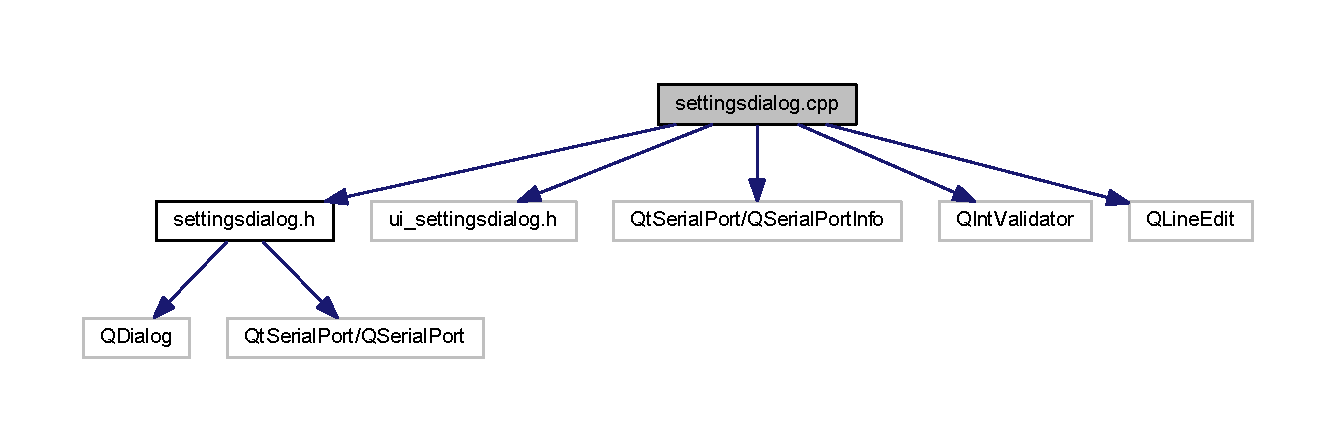
\includegraphics[width=350pt]{settingsdialog_8cpp__incl}
\end{center}
\end{figure}

\hypertarget{settingsdialog_8h}{}\section{settingsdialog.\+h File Reference}
\label{settingsdialog_8h}\index{settingsdialog.\+h@{settingsdialog.\+h}}
{\ttfamily \#include $<$Q\+Dialog$>$}\\*
{\ttfamily \#include $<$Qt\+Serial\+Port/\+Q\+Serial\+Port$>$}\\*
Include dependency graph for settingsdialog.\+h\+:
\nopagebreak
\begin{figure}[H]
\begin{center}
\leavevmode
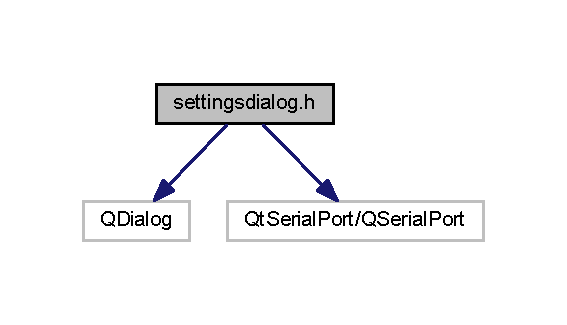
\includegraphics[width=272pt]{settingsdialog_8h__incl}
\end{center}
\end{figure}
This graph shows which files directly or indirectly include this file\+:
\nopagebreak
\begin{figure}[H]
\begin{center}
\leavevmode
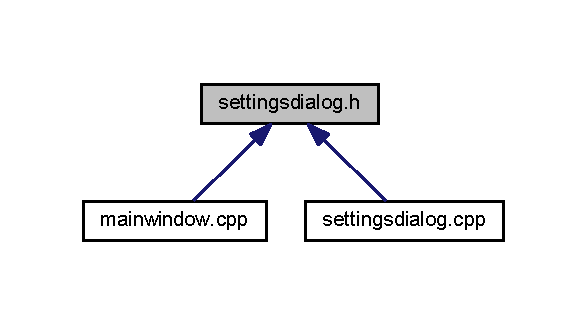
\includegraphics[width=282pt]{settingsdialog_8h__dep__incl}
\end{center}
\end{figure}
\subsection*{Classes}
\begin{DoxyCompactItemize}
\item 
class \hyperlink{class_settings_dialog}{Settings\+Dialog}
\item 
struct \hyperlink{struct_settings_dialog_1_1_settings}{Settings\+Dialog\+::\+Settings}
\end{DoxyCompactItemize}
\subsection*{Namespaces}
\begin{DoxyCompactItemize}
\item 
 \hyperlink{namespace_ui}{Ui}
\end{DoxyCompactItemize}

%--- End generated contents ---

% Index
\backmatter
\newpage
\phantomsection
\clearemptydoublepage
\addcontentsline{toc}{chapter}{Index}
\printindex

\end{document}
